\documentclass[12pt]{article}
\usepackage[margin=1in]{geometry}
\usepackage{amsmath}
\usepackage{amssymb}
\usepackage{graphicx}
\usepackage{stmaryrd}
\usepackage{float}

\author{Kyler Little\vspace{-0.6cm}}
\title{Homework \#5: Machine Learning\vspace{-0.3cm}}
\date{April 14, 2018\vspace{-0.7cm}}

\begin{document}
	\maketitle
	\section*{Problem \#1}
	Consider two finite-dimensional feature transforms $\Phi_1$ and $\Phi_2$ and their corresponding kernels $K_1$ and $K_2$. \\
	(a) Define $\Phi(x) = (\Phi_1(x), \Phi_2(x))$. Express the corresponding kernel of $\Phi$ in terms of $K_1$ and $K_2$. \\
	Firstly, it's important to note that $\Phi(x)$ is also finite-dimensional since both $\Phi_1(x)$ and $\Phi_2(x)$ are finite-dimensional. Next, it's a simple matter of linear algebra to derive the kernel. \\ $K(x,x')=\Phi(x)^T\Phi(x')=\left[\begin{array}{cc}\Phi_1(x)^T&\Phi_2(x)^T\end{array}\right]\left[\begin{array}{c}\Phi_1(x') \\ \Phi_2(x')\end{array}\right] = \Phi_1(x)^T \Phi_1(x') + \Phi_2(x)^T \Phi_2(x') = K_1(x,x')+K_2(x,x')$. 
	\\
	(b) Consider the matrix $\Phi_1(x) \Phi_2(x)^T$ and let $\Phi(x)$ be the vector representation of the matrix (say, by concatenating all the rows). Express the corresponding kernel of $\Phi$ in terms of $K_1$ and $K_2$. \\
	First, we need to find exactly what $\Phi$ is in this situation (i.e. what does it mean to concatenate rows). When we concatenate the rows, we simply put row 2 behind row 1, then row 3 behind row 2, and so on. We take the transpose of this vector so that it's a column vector. Now, let $u = \Phi_1$ and $v= \Phi_2$ to simplify the notation a bit. Also, assume $\Phi_1(x)$ has $n$ dimensions, and $\Phi_2(x)$ has $m$ dimensions. We have:
	\begin{align*}
		K(x,x') &= \Phi(x)^T\Phi(x') \\
		&= \text{concat}(\Phi_1(x) \Phi_2(x)^T)^T \text{concat}(\Phi_1(x') \Phi_2(x')^T) \\
		&= \text{concat}(uv^T)^T \text{concat}(u'v'^T) \\
		&= \sum_{i=1}^{m} \sum_{j=1}^{n} u_i v_j u'_i v'_j \\
		&= u^T u' v^T v' \\
		&= K_1(x,x') K_2(x,x')
	\end{align*}
	In this case, the kernel is simply the product of the other two kernels. \\
	(c) Hence, show that if $K_1$ and $K_2$ are kernels, then so are $K_1 + K_2$ and $K_1 K_2$. \\
	Assume otherwise. This means that it's not possible to find kernels $K_1+K_2$ and $K_1 K_2$ such that $K_1$ and $K_2$ are both separately kernels. However, we just did that in parts (a) and (b); thus, we have a contradiction. This means the original statement must be true. $\Box$
	
	\section*{Problem \#2}
	Exercise 8.16 (e-Chap:8-42) in LFD. Please ignore part (c) and only do (a), (b), (d). \\
	Exercise 8.16
	Show that the optimization problem in (8.30) is a QP-problem. \\
	(a) Show that the optimization variable is 
	$u =\left[\begin{array}{c}
		b\\
		w\\
		\xi
	\end{array}\right]$, where $\xi =\left[\begin{array}{c}
	\xi_1\\
	\vdots\\
	\xi_n
	\end{array}\right]$. \\
	Although I'm not exactly sure what this question is asking, I'm assuming that it means to demonstrate the minimization problems are identical (i.e. the QP form of the problem is equivalent to the minimization problem of 8.30). If we let the optimization variable be $u$, then we have:
		\begin{align*}
		\underset{u \in R^{1+d+N}}{\text{minimize}} &\qquad \frac{1}{2}u^T\text{Q}_D u+p^{T}u \\
		\text{subject to} & \qquad Au \ge C
		\end{align*}
	We need to show this is equivalent to 8.30. Using the $Q$ below, it's easy to see $\frac{1}{2}u^TQu = \frac{1}{2}w^Tw$ since the identity matrix within $Q$ grabs $w$ from within $u$ while the rest of the matrix $Q$ is zeros, removing $b$ and $\xi$. Using the $p$ below, we see that $p^T u = \sum_{i=1}^{N} C\xi_i = C\sum_{i=1}^{N} \xi_i$, exactly like 8.30.
	\\ 
	(b) Show that $u^* \leftarrow \text{QP}(Q,p,A,c)$, where \\
	$Q =\left[\begin{array}{ccc}
	0&0_d^T&0_N^T\\
	0_d&I_d&0_{d \times N}\\
	0_N&0_{N \times d}&0_{N \times N}
	\end{array}\right]$, $p =\left[\begin{array}{c}
	0_{d+1} \\
	C \cdot 1_N
	\end{array} \right]$, $A =\left[\begin{array}{cc}
	YX&I_N\\
	0_{N \times d+1}&I_N
	\end{array}\right]$, and $c =\left[\begin{array}{c}
	1_N \\
	0_N
	\end{array} \right]$,\\
	and $YX$ is the signed data matrix from Exercise 8.4. \\
	Again, the author is not exactly clear in what he wants to be done. From the problem statement, it appears that he wants me to demonstrate that the optimal $u$ is obtained by solving the QP-problem with the given inputs. Thus, I'm assuming this means I need to show the equivalence of conditions (i.e. $Au \ge C \leftrightarrow y_n(w^Tx_n+b \ge 1 - \xi_n) \ \text{and}\  \xi_i \ge 0$). \\
	To do so, I will start by explicitly writing out the $Au \ge C$.
	\begin{center}
	$\left[
	\begin{array}{ccccccc}
	y_1 & \cdots & y_1x_1^T & \cdots & 1 & \cdots & 0 \\
	\vdots & & \vdots & & 0 & \ddots & 0 \\
	y_N & \cdots & y_Nx_N^T & \cdots & 0 & \cdots & 1 \\
	0 & \cdots & 0 & \cdots & 1 & \cdots & 0 \\
	\vdots & & \vdots & & 0 & \ddots & 0 \\
	0 & \cdots & 0 & \cdots & 0 & \cdots & 1 \\
	\end{array}
	\right]
	\left[
	\begin{array}{c}
	b \\
	w \\
	\xi
	\end{array}
	\right]
	\ge
	\left[
	\begin{array}{c}
	1 \\
	\vdots \\
	1 \\
	0 \\
	\vdots \\
	0
	\end{array}
	\right]
	$
	\end{center}
	From here, if we perform the matrix-vector multiplication, we get the following result for the first $N$ rows: $y_i b + y_ix_i^Tw + \xi_i, \forall i \in {1, ..., N}$. This is equivalently $y_i (w^T x_i +b) \ge 1 - \xi_i, \forall i \in {1, ..., N}$. The last $N$ rows result in $\xi_i \ge 0, \forall i \in {1, ..., N}$. This exactly equals the problem in 8.30. Now, the problem is in standard QP form. Thus, to solve for the optimal hyperplane $u^*$, we merely solve the QP problem now.
	\\
	(d) How do you determine which data points violate the margin, which data points are on the edge of the margin and which data points are correctly separated and outside the margin? \\
	$\xi_i$ captures by how much $(x_i,y_i)$ fails to be separated. Specifically, if we have that $\xi_i = 0$ for a particular data point, then the margin is not violated and no loss occurs. The data point is correctly classified. This also means that $y_i(w^Tx_i + b) > 1$. If we have that $y_i(w^Tx_i + b) = 1$, then the data point is on the edge of the margin and again, $\xi_i = 0$. Thus, it is easy to see that $\xi_i$ captures how far into the margin a data point is, since non-zero $\xi_i$ means that the margin was violated (also meaning $y_i(w^Tx_i + b) < 1$).
		
	\section*{Problem \#3}
	(a) Describe what are hinge loss, logistic regression loss, and 0-1 loss mathematically. Describe their similarities and differences using the unified picture we developed in class. \\
	We start with 0-1 loss. \\
	Machine learning classification problems can be formulated as a ``minimizing the loss" problems. In general, suppose we have data points $x_1, x_2, ..., x_N \in R^d$ with corresponding classifications $y_1, y_2, ..., y_N \in \{-1,+1\}$. For the most general case, we classify by the sign of the linear signal. In other words, if $y_i(w^T x_i + b) \ge 0$, then a point is correctly classified. If the linear signal is negative, it's not correctly classified. We can formulate the idea of minimizing the loss by characterizing the problem as:
	 \begin{align*}
	 \underset{w, b}{\text{minimize}} &\qquad L_{0/1} (y_i(w^Tx_i + b)) \\
	 \text{where} &\qquad L_{0/1}(z) = 
	 	\begin{cases}
	 	1 & \text{if } z < 0 \\
	 	0 & \text{if } z \ge 0 \\
	 	\end{cases}
	 \end{align*}
	 In this way, the loss problem is formulated as minimizing the number of misclassified points. Individually, the 0-1 loss function assigns a value of 1 to a misclassified point and a value of 0 to a correctly classified point.
	\\
	Now what about logistic regression loss and hinge loss? We can use the same logic to define those loss functions. 
	In both SVM and logistic regression, the loss functions are already conveniently defined. For SVM, the hinge loss is defined to be:
	\begin{align*}
		L_{\text{hinge}} &= \text{max}(0, 1-z) \ \text{where} \\
		z&= y_i(w^Tx_i+b)
	\end{align*}
	In this loss function, a correctly classified point must satisfy the condition: $y_i(w^Tx_i+b) \ge 1$ due to how the SVM problem is formulated. This loss function assigns a value of $1-y_i(w^Tx_i+b)$ or $1-z$ to a misclassified point and a value of 0 to a correctly classified point. \\
	Lastly, we look at the logistic regression loss function. Again, it is already conveniently defined by the cross-entropy term. It is defined to be:
		\begin{align*}
		L_{\text{logistic}} &= \log_2(1+\exp^{-z}) \ \text{where} \\
		z&= y_i(w^Tx_i+b)
		\end{align*}
	In this case, classified and misclassified points are actually treated the same since the loss function is not piecewise. Both are assigned values: $\log_2(1+\exp^{-y_i(w^Tx_i+b)})$. This means that correctly classified points result in a small loss while misclassified points result in a large loss. We can visualize all three loss functions with the graph below. Note: I borrowed this from the notes online, so it includes an extra loss function not discussed in this homework (the modified huber loss).
	\begin{figure}[h]
		\begin{center}
			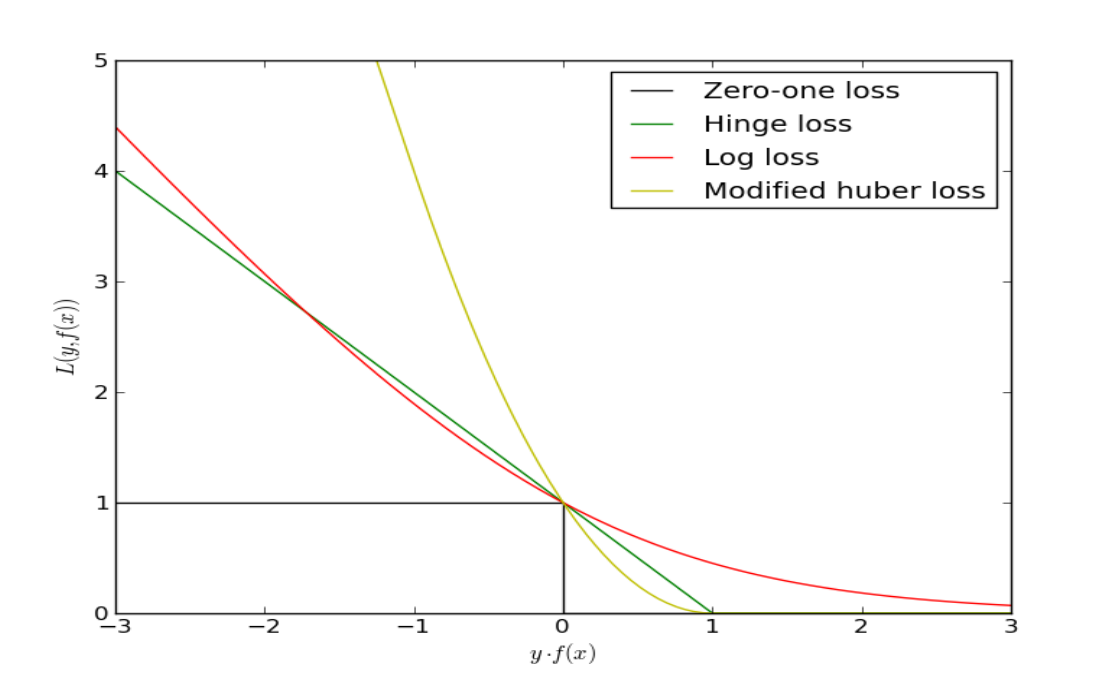
\includegraphics[width=5in]{unified_loss.png}
			\caption{An overview of different loss functions}
			\label{fig:sigmoidEx}
		\end{center}
	\end{figure}
	\\
	(b) By relying on the result in the above question, consider a point that is correctly classified and distant from the decision boundary. Why would SVM’s decision boundary be unaffected by this point, but the one learned by logistic regression be affected? \\
	The SVM's decision boundary is unaffected because the SVM only cares about support vectors (points that are on the decision boundary). In fact, non-support vectors are not even used in the calculation of the margin in SVM. Thus, SVM's decision boundary is completely unaffected by that point. On the other hand, logistic regression is still affected. This is because the goal of logistic regression is to maximize the likelihood that all points are correctly classified. Thus, it needs to take into consideration all points in order to do so. 
	
	\section*{Problem \#4}
	Summarize your observations from the coding portion into a short report. In your report, please report the accuracy result and total support vector number of each model. A briefly analysis based on the results is also needed.
	
	
\end{document}